% =====================================================================================
\section{Results: patterns, errors and focusing}
\label{sec:other}
% =====================================================================================

\subsection{Usable phase patterns}
\label{sec:modes}

To find what each structure can do at best, we place a heater under every emitter, so that $G$ is $N\times N$, and
remove the free offset. The singular value decomposition $G=U\Sigma V^{\mathsf T}$ gives independent phase patterns
$\bm u_i$ with gains $s_i$ (rad/W); the power for a given amount of pattern $i$ scales as $1/s_i$. A pattern is
counted as usable if it costs at most ten times the cheapest ($s_i\ge0.1\,s_1$).

On the \stack{standard} stack at \qty{2}{\micro\metre} pitch, \num{15} of \num{32} patterns are usable, and all cost
about the same: the heaters act as independent phase shifters. On the membranes the gains fall steeply: \num{4} patterns are usable on the \stack{undercut}, \num{3} on the \stack{slot} and \num{2} in
\stack{vacuum}. For a kernel that depends only on $x-\xh$, the singular vectors approach Fourier modes of spatial
frequency $q_m\approx\pi m/(Nd)$ and the gains approach the kernel's Fourier transform. For a Gaussian kernel of
half-width $\Lth$ the gains fall as $\exp(-q^2\Lth^2/4\ln2)$, so the number of patterns above the threshold is
\begin{equation}
  M \;\approx\; \frac{\sqrt{2\ln 10}\,\sqrt{2\ln 2}}{\pi}\,\frac{N d}{\Lth}\;\approx\;0.80\,\frac{N d}{\Lth}.
  \label{eq:modecount}
\end{equation}
This predicts \num{11.8}, \num{15.8} and \num{31.6} for pitches of \num{1.5}, \num{2} and \qty{4}{\micro\metre}; the
computed counts are \num{11}, \num{15} and \num{32}.

The cheapest patterns on the membranes are their simplest steady states: a ramp (heater to sink)
and a dome (between two sinks). On the one-sided \stack{slot} and \stack{vacuum} membranes the ramp is cheapest; on
the two-walled \stack{undercut} the dome and ramp cost the same. These are exactly the two patterns used for steering
and focusing, and the third pattern already costs \numrange{4}{14} times more. Since heaters can only heat, the
\stack{vacuum} membrane cannot even form the dome: all its heater profiles rise monotonically towards the slot, so
any combination with $P_k\ge0$ is monotonic.

As a direct test, each structure was asked to split the beam into two at $\pm\theta$ with all \num{33} heaters. The
\stack{standard} stack reaches the ideal efficiency of the finite array (\numrange{0.62}{0.76} of the light in the
two beams). The membranes reach at most \num{0.46} at \ang{\pm 3} and less than \num{0.03} at \ang{\pm 5} or more,
because the required phase features ($\lambda/\sin\theta$, \qty{9}{\micro\metre} at \ang{10}) are narrower than their
\qtyrange{20}{30}{\micro\metre} spreading. The arrangement best suited to sharp patterns is therefore short spreading
($\Lth/d\lesssim2$) with a heater under every emitter, which is the conventional design.
\subsection{Fabrication errors}
\label{sec:fab}

Each waveguide carries a static phase error from width and thickness variations. We model the errors as Gaussian
with rms $\sigma$ and correlation $\exp(-\Delta x^2/2\ell^2)$ between waveguides $\Delta x$ apart; $\ell=0$ is the
independent case. Measured silicon-photonic variation has a smooth wafer-scale part (about \qty{80}{\percent} of the
width variance) and a local part uncorrelated between sites~\cite{xing2023}; the local part accumulates along a
waveguide as $\sigma^2\approx L/L_\mathrm{coh}$, with $L_\mathrm{coh}=\qty{4.17}{\milli\metre}$ for strip
waveguides~\cite{yang2015}. Three cases are compared by Monte Carlo: uncorrected, corrected by refitting the heaters
with \cref{eq:nnls}, and trimmed (error removed).

\paragraph{Independent errors.} For independent Gaussian errors the mean Strehl ratio of \cref{eq:strehl} is
\begin{equation}
  \langle S\rangle \;=\; \ee^{-\sigma^{2}} + \frac{1-\ee^{-\sigma^{2}}}{N},
  \label{eq:ruze}
\end{equation}
since the $N$ diagonal terms of $|\sum_n\ee^{\ii\varepsilon_n}|^2$ equal one and each off-diagonal term averages to
$\ee^{-\sigma^2}$~\cite{ruze1966}. After correction every design stays on this curve (\cref{fig:ruze}a): at
$\sigma=\qty{1}{\rad}$ the corrected Strehl ratio is \numrange{0.39}{0.43}, against \num{0.39} without correction. A
fit onto $K$ heater profiles plus the offset removes on average only $(K+1)/N$ of the variance of independent noise:
\qty{6}{\percent} for one heater, \qty{12}{\percent} for three.

\paragraph{Smooth errors.} Errors correlated over $\ell\gtrsim\qtyrange{16}{32}{\micro\metre}$ consist mainly of
offset, gradient and curvature, which the heaters can produce, and are corrected. At
$\ell=\qty{32}{\micro\metre}$ and $\sigma=\qty{1}{\rad}$, one heater raises $S$ from \num{0.78} to \num{0.96}, at an
extra power below \qty{0.2}{\milli\watt}.

\paragraph{Static trim.} Without trim, $S\ge0.9$ limits each waveguide's independent path to
$-L_\mathrm{coh}\ln0.9=\qty{0.44}{\milli\metre}$. A \ang{10} heated section kept below \qty{60}{\kelvin} is already
\qty{1.04}{\milli\metre} long, which alone limits an untrimmed array to $S\approx0.78$ (\cref{fig:ruze}b). The design
therefore requires a one-time static trim of each waveguide's phase beyond small angles. Trimming has been
demonstrated on ring resonators~\cite{jayatilleka2021} but, to our knowledge, not on an OPA. With trim, the
comparison with a conventional array is a one-time trim plus $K$ wires against $N$ wires plus a calibration for each
beam direction, which takes from \qty{40}{\second} to an hour per beam~\cite{lian2024}.

\begin{figure}[htbp]
  \centering
  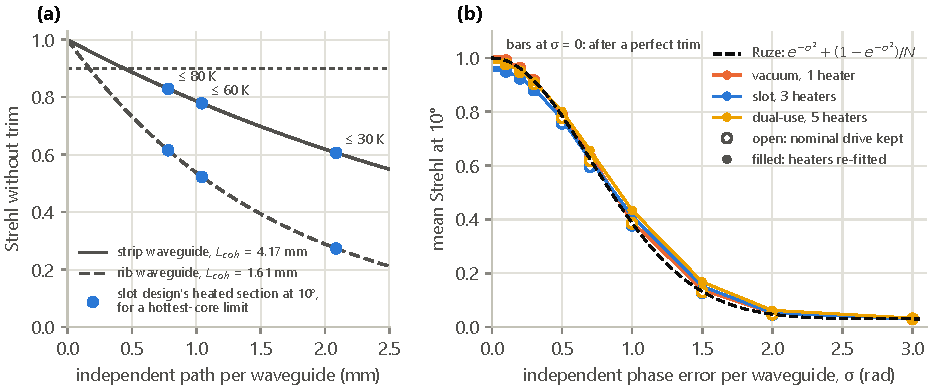
\includegraphics[width=\linewidth]{rep_ruze}
  \caption{Independent phase errors. (a)~Mean Strehl ratio at \ang{10} against rms error, uncorrected and corrected
  by the heaters, with \cref{eq:ruze}. (b)~Without trim: Strehl ratio against independent path length, with the
  heated-section length at \ang{10} for three limits on the hottest core.}
  \label{fig:ruze}
\end{figure}
\subsection{Tunable lens}
\label{sec:lens}

In vacuum the membrane temperature obeys $\kt\,T''=-q$, with $q$ the heater power per unit area. A parabola requires
$T''$ constant, which is produced by heat deposited uniformly across the array between two cold walls. For a heater
of width $W=2X$ carrying $P/\Lh$ per unit length, $q=P/(\Lh W)$ and, by symmetry, $T(0)-T(x)=qx^2/(2\kt)$ over the
heated strip: an exact parabola. The lens strength is $a=\gamma\Lh[T(0)-T(X)]$, so the power per radian is
\begin{equation}
  \frac{P}{a} \;=\; \frac{2\,\kt\,W}{\gamma\,X^{2}} \;=\; \qty{0.89}{\milli\watt\per\rad}
  \qquad (W=\qty{64}{\micro\metre},\ X=\qty{32}{\micro\metre}).
  \label{eq:lenspower}
\end{equation}
Since $\dndT>0$, heating the centre lengthens its optical path and the lens converges. A parabola needs cold walls
on both sides, so the lens uses the \stack{undercut} membrane rather than the slotted one.

\Cref{fig:lens} shows the result in a two-dimensional scalar simulation of the light above the array, with each
emitter a line source carrying the phase the heaters produce. Asked for a lens of $f=\qty{0.15}{\milli\metre}$, a single
narrow centre heater produces a tent of phase rather than a parabola, and the light spreads into a long streak with
only \num{0.22} of a perfect lens's intensity at the focus (\cref{fig:lens}a). One heater as wide as the array produces
the parabola of \cref{eq:lenspower} and a focus indistinguishable from a perfect lens (\cref{fig:lens}b). The light
reaching the focus agrees with the Strehl ratio computed from the phase error to within \num{0.016} at every focal
length tested, so the Strehl ratio is used to judge the lens.

The wide heater costs \qty{1.16}{\milli\watt\per\rad} in air (\num{0.89} in vacuum) and remains a good lens down to
$f\approx\qty{35}{\micro\metre}$, beyond the paraxial range of \cref{eq:lens}. A lens of $f=\qty{1}{\milli\metre}$ therefore
needs about \qty{2.4}{\milli\watt} and only \qty{2.5}{\kelvin} between centre and edge. The centre heater is cheaper,
\qty{0.56}{\milli\watt\per\rad}, but is usable only for $f\ge\qty{0.38}{\milli\metre}$. Isolated heaters can wrap a lens
(a Fresnel lens), so their power stops growing at about $a=2\pi$, while ours grows in proportion to $a$
(\cref{fig:lens}c). For weak lenses ($f\gtrsim\qty{0.5}{\milli\metre}$) ours is \numrange{8}{16} times cheaper than
isolated heaters with the same $\Ppi$, and \numrange{3}{6} times cheaper than the best single-pass suspended
heaters~\cite{fang2011}; the two cross at $f\approx\qty{0.15}{\milli\metre}$.

A layout cannot be optimal for both jobs: the best lens layouts have no heater at the array ends and cannot steer.
Five heaters at 0, $\pm16$ and $\pm\qty{33}{\micro\metre}$ do both. They steer \ang{\pm 22.8} at \qty{5.4}{\mWdeg}, four
times the power of the \stack{slot} design, and focus to $f=\qty{0.15}{\milli\metre}$ on axis or at \ang{10} with $S$ of
\num{0.93} and \num{0.90} (\cref{fig:lens}d--f); at any angle they focus down to $f\approx\qtyrange{90}{115}{\micro\metre}$.

\begin{figure}[htbp]
  \centering
  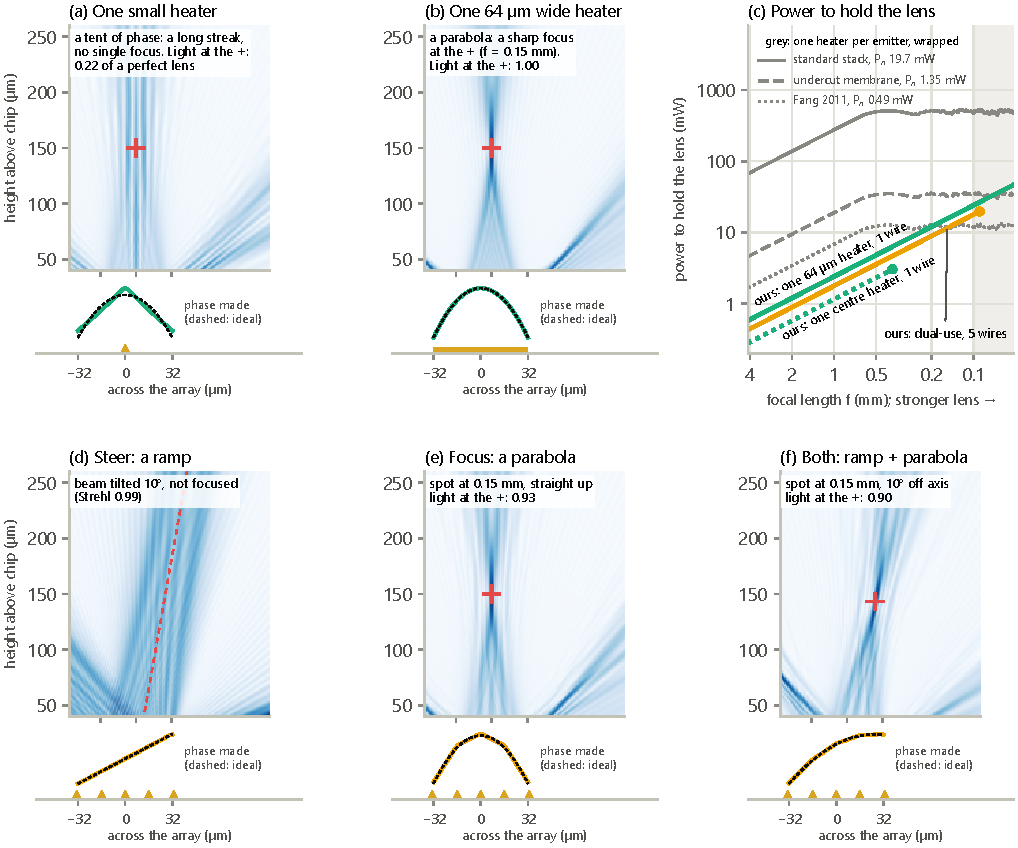
\includegraphics[width=\linewidth]{rep_lens}
  \caption{The thermal lens on the \stack{undercut} membrane. (a,~b,~d--f)~Two-dimensional scalar simulation of the
  light above the array (square-root intensity scale); the cross marks the focus of a perfect lens, and the strip
  below each map shows the phase produced (solid) against the target (dashed), with the heaters in gold.
  (a)~One narrow centre heater and (b)~one \qty{64}{\micro\metre} heater, both asked for $f=\qty{0.15}{\milli\metre}$.
  (c)~Power to hold a lens against focal length; grey, one isolated heater per emitter with wrapped phases at three
  values of $\Ppi$; shaded, $f<\qty{0.1}{\milli\metre}$, where the paraxial form is approximate. (d--f)~The five-heater
  layout steering to \ang{10}, focusing, and both at once. The faint diagonal streaks are grating lobes.}
  \label{fig:lens}
\end{figure}

\subsection{Nonlinearity at high temperature}
\label{sec:nonlinear}

Because the ramp cannot be wrapped, the hottest core is about \qty{62}{\kelvin} above ambient at \ang{10}, beyond the
range in which the linear model is accurate to \qty{1}{\percent} (about \qty{30}{\kelvin}). With temperature-dependent
conductivities the true rise falls below the linear prediction by \qty{2.4}{\percent} at \qty{80}{\kelvin} and
\qtyrange{6}{7}{\percent} at \qty{185}{\kelvin} (\cref{fig:nonlinear}a), because oxide, which carries the heat,
conducts better when hot.

This departure follows a simple law. For conductivity $k=k_0(1+\beta\Delta T)$, the Kirchhoff transform
$\vartheta=\Delta T+\beta\Delta T^2/2$ satisfies $k_0\nabla\vartheta=k\nabla T$ and hence obeys the linear equation with
the same sources and boundary values~\cite{carslaw1959}. The linear model therefore gives $\vartheta$ exactly, and to
first order
\begin{equation}
  \Delta T \;=\; \vartheta - a\,\vartheta^{2}, \qquad a=\beta/2 .
  \label{eq:kirchhoff}
\end{equation}
With $a=\qty{3.0e-4}{\per\kelvin}$ on the membrane and \qty{3.5e-4}{\per\kelvin} on the \stack{standard} stack,
\cref{eq:kirchhoff} reproduces every nonlinear profile to within \qty{0.25}{\percent} of the peak, and the two-heater
runs to \qty{0.14}{\percent}. Any drive can therefore be evaluated by superposing linearly and applying
\cref{eq:kirchhoff}. Silicon's thermo-optic coefficient also rises with temperature~\cite{cocorullo1999}, which acts in
the opposite direction; its relative rate $b$ could not be confirmed from the original paper and is bracketed between
0 and \qty{1.4e-3}{\per\kelvin}.

When the heater powers are fitted to the true, nonlinear response, as a calibration on a real device would do, the
beam quality is nearly unchanged (\cref{fig:nonlinear}b). For the \stack{slot} design with \qty{1}{\milli\metre}
heaters, $S$ at \ang{10} is \numrange{0.95}{0.97} against \num{0.96} for the linear model, and the drive differs from
the linear one by about \qty{2}{\percent}. At \ang{20} (\qty{120}{\kelvin}) $S$ is \numrange{0.81}{0.89}. The
nonlinearity is therefore a calibration matter, not a limit on the design, up to about \ang{20} with
\qty{1}{\milli\metre} heaters; longer heaters reduce the temperature in proportion.

\begin{figure}[htbp]
  \centering
  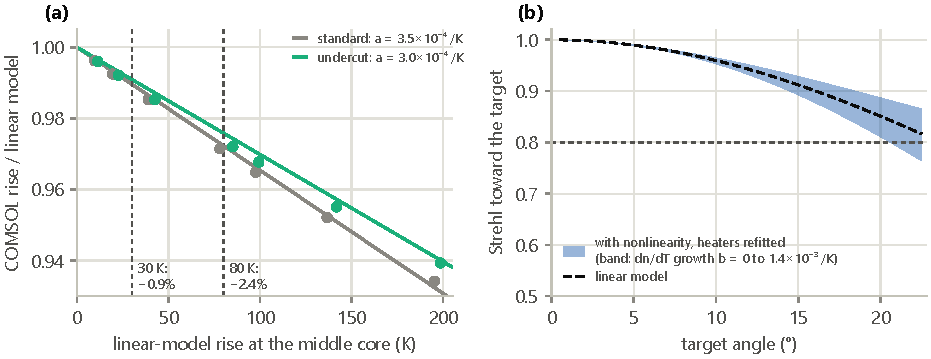
\includegraphics[width=\linewidth]{rep_nonlinear}
  \caption{Nonlinearity. (a)~True temperature rise divided by the linear prediction, with the law of
  \cref{eq:kirchhoff}. (b)~Strehl ratio of the \stack{slot} design (\qty{1}{\milli\metre} heaters) with the heater
  powers fitted to the nonlinear response, for the range of $b$, against the linear model. The hottest core reaches
  \qty{30}{\kelvin} at \ang{4.8} and \qty{80}{\kelvin} at \ang{13.2}.}
  \label{fig:nonlinear}
\end{figure}

\subsection{The grating axis}
\label{sec:gratingaxis}

Along the waveguides the emission angle follows the grating equation,
\begin{equation}
  \sin\theta_y \;=\; \neff^{\mathrm{g}} - \frac{\lambda}{\Lambda},
  \label{eq:grating}
\end{equation}
with $\Lambda$ the period and $\neff^{\mathrm g}$ the effective index of the grating section. The grating model gives
\ang{9.64} at the design point and rates of $+\ang{1.90}$ per \qty{10}{\nano\metre} of period, $+\ang{1.16}$ per
\qty{100}{\kelvin}, and $-\ang{0.150}$ per nanometre of wavelength after correction for the strip's group index
(\cref{fig:grating}); all \num{18} runs lie within \ang{0.03} of \cref{eq:grating}. Tuning the laser from
\qtyrange{1500}{1600}{\nano\metre} sweeps the beam by about \ang{15} along the grating, which together with the
\ang{\pm 22.8} across the array gives a two-dimensional field of view. The temperature sensitivity is also why the
heaters sit before the gratings: steering heaters over a grating would be limited to its \qty{110}{\micro\metre}
emission length, requiring about \qty{370}{\kelvin} at \ang{10} and tilting the beam by about \ang{4} along the
grating.

\begin{figure}[htbp]
  \centering
  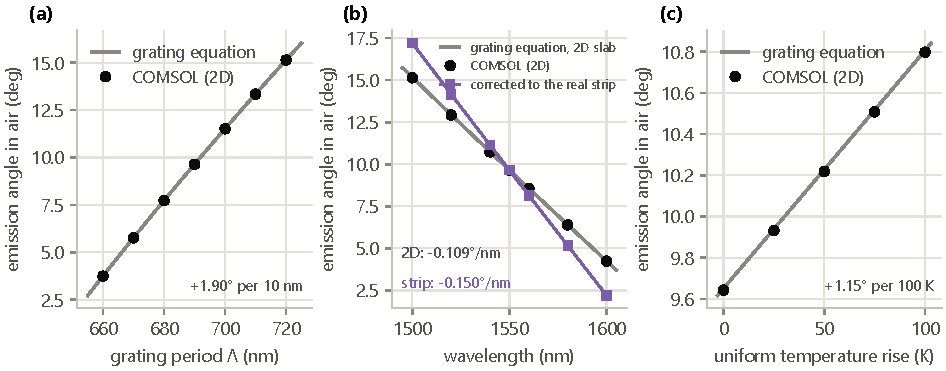
\includegraphics[width=\linewidth]{rep_grating}
  \caption{Grating model: emission angle against (a)~period, (b)~wavelength, with the correction for the strip's
  group index, and (c)~temperature. Grey lines are the grating equation with nothing fitted.}
  \label{fig:grating}
\end{figure}
